\clearpage
\subsubsection{Brief introduction to COCOMO II}
COCOMO (COnstructive COst MOdel) is a cost estimation algorithm allowing to estimate the time, effort and money needed to develop a project. It provides an empirical non-linear model based on two series of values:
\begin{itemize}
	\item\textbf{Scale Factors}, providing a gross estimate of the effort needed for the project.
	\item\textbf{Cost Drivers}, which can be \textit{Early Design} or \textit{Post-Architecture} and are applied to the effort as a multiplier.
\end{itemize}
COCOMO was originally published in 1981, based on a study of 63 projects of varying size and languages. COCOMO II, published in 2000, extends COCOMO by savoiding several underlying assumptions, such as waterfall development and stable requirements, and separating \textit{Early Design} from \textit{Post-Architecture} effort multipliers.

The general formula for calculating the needed Person-Months is $$ PM = 2.94 \cdot Size^E \cdot \prod_{i=1}^{n} EM_i $$ where $$ E = 0.91 + 0.01 \cdot \sum_{i=1}^{5}ScaleFactor_i $$ and size is expressed in Kilo Source Lines of Code, possibly derived from Function Points.

This estimate is made after planning the architecture, so we will use the \textit{Post-Architecture} model.

\subsubsection{Scale Factors}
\paragraph*{Precedentedness: Low}
We have never built any similar application, although the structure of the application is not different from other projects that we have worked on.

\paragraph*{Development Flexibility: High}
Management did not impose a choice of framework, architecture or any set of constraints except the product goals.

\paragraph*{Architecture/Risk Resolution: Low}
We were not provided with little information about risk management, budget and architecture, and had to work it out ourselves.

\paragraph*{Team Cohesion: High}
We had a couple of small misunderstandings early on, but managed to work them out and have been efficiently working together.

\paragraph*{Process Maturity: Nominal}
We believe the CMMI level to be around "Defined", accounting for our relative lack of experience but proactive attitude.

\subsubsection{Post-architecture Cost Drivers}
\paragraph*{Required Software Reliability: Nominal}
A service malfunction could cause inconvenience and non-trivial financial losses.

\paragraph*{Data Base Size: Nominal}
The database size is standard for a medium-to-small-sized application. The database mainly stores data about Cars, Users, and Parking Areas.

\paragraph*{Product Complexity: Nominal}
The product's complexity is par for the course for a medium-to-small-sized application.

\paragraph*{Developed for Reusability: Nominal}
There was no specific reusability requirement, but we made the application modular, so to allow for future expansion and modification.

\paragraph*{Documentation Match to Lifecycle Needs: Nominal}
Adequately-sized documentation is provided for the various stages of the project.

\paragraph*{Analyst Capability: Nominal}
We believe our skills to be around average, accounting for our relative lack of work experience.

\paragraph*{Programmer Capability: Nominal}
We believe our skills to be around average, accounting for our relative lack of work experience.

\paragraph*{Personnel Continuity: Very High}
The three of us kept working on the project from beginning to end.

\paragraph*{Application Experience: Low}
We have little experience in developing complete applications.

\paragraph*{Platform Experience: Low}
We have little experience working with Spring, Tomcat and nginx.

\paragraph*{Language and Toolset Exerience: Nominal}
We have a good undersdtanding of Java, if a somewhat limited experience.

\paragraph*{Time Constraint: Very High}
Rapid communication between the Cars, the User Application and the Central Service is essential for good software performance.

\paragraph*{Storage Constraint: Nominal}
No specific storage constraint was mentioned, and the amount of data created by the application is modest in size.

\paragraph*{Platform Volatility: Low}
No major or minor changes to the platform were observed during the project.

\paragraph*{Use of Software Tools: High}
During development, several strong tools would be used to check on the lifecycle, such as mantaining a git repository.

\paragraph*{Multisite Development: Extra High}
Most of the work was done from home, coordinating through IRC.

\paragraph*{Required Development Schedule: Nominal}
A rigid schedule was imposed on us for the first documents (RASD and DD), but we had more freedom for the project development.

\subsubsection{Effort Calculation}
By applying the algorithm (we used a free online tool, available at \\\texttt{http://csse.usc.edu/tools/COCOMOII.php}) based on our estimate of 236 FP, we obtained a result of 37.6 Person-Months, equivalent (considering a 160-hours work week) to 6016 Person-Hours.
\begin{figure}[h]
	\centering
	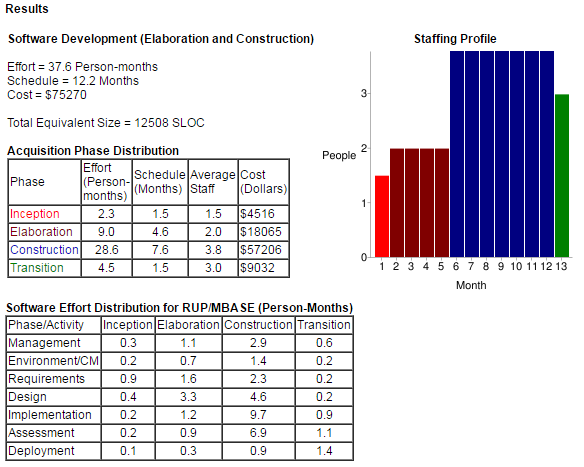
\includegraphics[width=\textwidth]{Images/COCOMO}
	\caption{COCOMO tool results}
\end{figure}

\subsubsection{Scheduling}
COCOMO provides an estimate of the project time frame through the formula $$ Duration = 3.67 \cdot Effort^{SE} $$ where $$ SE = 0.28 + 0.2 \cdot (E - 0.91) $$
resulting in an estimate of 12.2 months.

\subsubsection{Team Dimension}
The dimension of the team can be easily calculated as $\frac{Effort}{Duration}$, which, in our case, yields a result of 3.1. Since there are 3 of us, the duration will likely be extended.

This is also due to the fact that the amount of staff needed in the different phases of development is not constant: the construction phase would optimally require 4 people working. This can be avoided by hiring an additional developer, or extending the deadline. In the latter case, a realistic adjusted duration would be equivalent to 14.2 months, to reflect the increased time needed for the software construction.